% SPDX-FileCopyrightText: Copyright (c) 2026 NVIDIA CORPORATION & AFFILIATES. All rights reserved.
% SPDX-License-Identifier: Apache-2.0
%
% ROLE: answer, in order: which configurations were selected; does the learned policy beat the best
%   baseline on held-out data (headline, exact scoped wording); where does it win and lose, including
%   unseen worker counts; do richer models help; what did it learn; does the result survive SLO
%   changes, router-state lag and timing perturbation; what the secondary comparisons and the AIS
%   league add; how much of the margin an in-class heuristic carries. Figures that duplicate a table,
%   the cache-pressure trend, the rung-to-rung table, robustness details, herding guards and the cost
%   table live in appendix-results.tex (app:results); the AIS league in appendix-ais-league.tex
%   (app:ais-league, sec:res-ais); the selected-row N and family tables in appendix-tables.tex.
% EVIDENCE: CR/facts/{finalists,test_results,robustness,secondary_metrics_test,
%   fairness_in_class_heuristic,tierA,tierBC}.json; CR/report/REPORT.md and CR/report/data/ (the
%   generated tables under generated/ are copied from report/data/tables/*.md by
%   scripts/make_tables.py); CR/audits/final/*.md.
% CI NOTE: generated tables carry the report's 10,000-draw segment bootstrap (fixed seed). The
%   headline facts file's own bootstrap gives [0.0150, 0.0498] for the headline segment mean, against
%   the report's [0.0150, 0.0501]; the difference is resampling noise. The text quotes the report's.
% STATUS: final for the simulation results. Everything here is AIS-timed replay, except the live-run
%   numbers that limit 5 quotes from sec:live. How the result tables are produced (copied from the
%   final report's fragments) is stated once, in app:repro.

\section{Results}
\label{sec:results}

Apart from the live-run numbers that limit 5 below quotes from \cref{sec:live}, every number in this
section comes from AIS-timed offline replay. Intervals are 95\%
percentile intervals from a bootstrap that resamples whole test segments with all their cells; where
a stratum has fewer than three segments, cells are resampled within each segment instead, marked
$\dagger$, and those intervals are optimistic because cells of one segment are not independent. Only
the pre-registered headline is a test; every other $p$-value is descriptive.
% src: CR/report/data/report_data.json method (10,000 draws, fixed seed; dagger rule)

% =====================================================================================
\subsection{Selection: the finalists}
\label{sec:res-selection}

Each policy's configuration was chosen on validation replicates $\krep = 0,1,2$ over its three
restarts and their checkpoints. The cross-policy choices were then made on fresh replicates
$\krep = 3,\dots,10$, by the same rule for baselines and learned arms, and the list of finalists was
frozen before the first test record was written.
\begin{itemize}
  \item \textbf{Best baseline.} Tuned \policy{ramjet}, 0.1411, ahead of \policy{ramjet} with a tuned
    queue threshold (0.1405) and \policy{llm-d-precise-prefix} (0.1393). The choice between
    \policy{ramjet} and \policy{llm-d-precise-prefix} was a near tie: \policy{ramjet} led by 0.0018
    in the mean over cells but trailed by 0.0087 in the mean over segments, so the comparison with
    \policy{llm-d-precise-prefix} was registered as a secondary before the test pass.
  \item \textbf{Headline learned arm.} M1-v2, 0.1783, ahead of M1-noaff (0.1692), M1 with a tuned
    queue threshold (0.1684), M2 rank 2 (0.1677) and M1 (0.1656). Its configuration is the
    best-so-far sample at generation 20 of the restart that started from the default router
    ($\theta = -\basis{0}$). On the fresh replicates it led \policy{ramjet} by $+0.0372$ per cell and
    $+0.0290$ per segment, on 5 of 6 validation segments.
  \item \textbf{Multiplicity.} 314 learned variants were validated over the study (every
    validation checkpoint of every learned run, the pilot and the post-hoc variants); 5 learned arms
    competed for the headline.
\end{itemize}
% src: CR/facts/finalists.json rankings_val_k3_10 (baseline_pool, learned_pool), headline
%      (learned m1v2@p2-m1v2-s1-g20-best_so_far, val_k3_10_margin: cell 0.03717, segment 0.02896,
%      5/6 segments), secondary_comparisons; CR/facts/tierBC.json decisions.val_best_baseline
%      (+0.0018 cell, -0.0087 segment); CR/facts/test_results.json lr11 (314; 5)

% =====================================================================================
\subsection{Headline: M1-v2 against the best baseline}
\label{sec:res-headline}

\begin{center}
\fcolorbox{black!40}{black!3}{\parbox{0.92\linewidth}{\small
\textbf{Headline.} In AIS-timed simulation, the learned router M1-v2
beats the branch's ported heuristics, each tuned with an equal budget. Against the
validation-selected best baseline, tuned \policy{ramjet}, its windowed goodput on the 60 frozen
test cells is higher by a segment-mean clipped log-ratio of $+0.0316$ (95\% segment-bootstrap
interval $[+0.0150, +0.0501]$; geometric-mean ratio 1.032, interval $[1.015, 1.051]$). It is ahead
on 10 of 12 independent test segments: all 8 non-session segments and 2 of the 4 session segments.
All four session segments tie at ceiling, with differences below 0.001 of either sign. The pre-registered
one-sided exact Wilcoxon test gives $p = 0.0017$, and
$\Pr(\text{M1-v2} \succ \text{ramjet}) = 0.833$ with interval $[0.583, 1.0]$, significant and
meaningful by the registered rule.}}
\end{center}
% src: CR/facts/test_results.json report_must_state MS-RH2-F1-scope (wording), headline
%      (segment_mean 0.031555, segments_ahead 10, wilcoxon 0.001709, p_greater 0.8333 [0.5833, 1.0],
%      geomean 1.0321 [1.0151, 1.0510], by_segment sessions:s6..s9 -0.0000146, -0.0000974, +0.0000453,
%      +0.000594); interval [0.0150, 0.0501] from CR/report/REPORT.md section 1
%      and generated/strata.tex (the facts file's own bootstrap: [0.0150, 0.0498])
% prov: MS-RH2-F1-scope (the box was titled "Headline, as the final audit allows")

\Cref{tab:headline} shows the twelve units the test counts (\cref{fig:headline} in
\cref{app:results} plots them). The claim was pre-registered,
evaluated once, reproduced bit for bit from the raw per-request rows by an independent auditor, and
not refuted by the robustness and simulator-dependence audit. It survives leaving out any one
segment (largest $p$ 0.0034), any one family (largest $p$ 0.027), the $\Nw = 6$ cells and the
FAST25 conversation cells; with the latter removed the segment mean is $+0.026$ and $p$ is unchanged.
% src: CR/audits/final/refute-headline-1.md (bit-for-bit reproduction; leave-one-segment-out max p
%      0.0034; drop-family max p 0.027; excluding N6 / conv cells); CR/report/REPORT.md section 3.3
%      ("Without them, the headline is +0.026 with p 0.0017 unchanged")

\begin{table}[tbp]
  \centering\small
  \caption{The headline per test segment: $\segstat_{\seg}$ (\cref{eq:segstat}), the mean over the
    segment's cells and replicates $\krep = 0,1,2$ of the clipped log-ratio of M1-v2's windowed
    goodput against tuned \policy{ramjet}'s.}
  \label{tab:headline}
  % src (D_omega): CR/facts/test_results.json headline.by_segment; (cells, modes): CR/cells/test.jsonl
  %      metadata (FAST25 conversation cells: 2 in w3, 1 in w5); statistics: headline
  \begin{adjustbox}{max width=\linewidth}
  \begin{tabular}{@{}llrlr@{}}
    \toprule
    Segment & Family & Cells & Load modes (cells) & $\segstat_{\seg}$ \\
    \midrule
    w3 & Mooncake 11, FAST25 conv.\ 2 & 13 & open 11, closed 2 & $+0.0668$ \\
    w5 & Mooncake 14, FAST25 conv.\ 1 & 15 & open 9, closed 6  & $+0.1009$ \\
    s6 & sessions & 6 & open 6           & $-0.0000$ \\
    s7 & sessions & 2 & open 1, closed 1 & $-0.0001$ \\
    s8 & sessions & 2 & open 1, closed 1 & $+0.0000$ \\
    s9 & sessions & 5 & open 1, closed 4 & $+0.0006$ \\
    T1 & AgentX & 4 & lanes 4 & $+0.0366$ \\
    T2 & AgentX & 2 & lanes 2 & $+0.0309$ \\
    T3 & AgentX & 5 & lanes 5 & $+0.0397$ \\
    T4 & AgentX & 3 & lanes 3 & $+0.0426$ \\
    x0 & FAST25 synthetic & 2 & open 1, closed 1 & $+0.0556$ \\
    x1 & FAST25 synthetic & 1 & open 1 & $+0.0051$ \\
    \midrule
    \multicolumn{4}{@{}l}{Segment mean (SE)} & $+0.0316$ (0.0093) \\
    \multicolumn{4}{@{}l}{One-sided exact Wilcoxon signed-rank $p$, 12 segments} & 0.0017 \\
    \multicolumn{4}{@{}l}{$\Pr(\text{M1-v2} \succ \text{ramjet})$ over segments, 95\% interval} & 0.833 $[0.583, 1.0]$ \\
    \multicolumn{4}{@{}l}{Geometric mean of segment ratios, 95\% interval} & 1.032 $[1.015, 1.051]$ \\
    \multicolumn{4}{@{}l}{Interquartile mean of segment ratios, 95\% interval} & 1.026 $[1.005, 1.050]$ \\
    \multicolumn{4}{@{}l}{Mean over cells (SE); cells ahead} & $+0.0506$ (0.0117); 50 of 60 \\
    \bottomrule
  \end{tabular}
  \end{adjustbox}
\end{table}
% src: CR/facts/test_results.json headline (by_segment; segment_se 0.009332; iqm 1.0264 [1.0054, 1.0503];
%      cell_mean 0.050584, cell_se 0.011666, cells_ahead 50)

\paragraph{Limits that travel with the headline.}
Five limits bound the headline.
% prov: the final audit's report_must_state items (CR/facts/test_results.json)
\begin{enumerate}
  \item \textbf{Only the sign is a claim.} The effect is below the pre-registered minimum detectable
    effect (0.038) and below the spread that timing perturbations induce (0.060). Its magnitude
    depends on the perturbation (\cref{sec:res-robustness}).
  \item \textbf{It is not ``learning beats every heuristic''.} The baseline pool lacks faithful
    LMetric, which lies inside M1-v2's class; added to the default cost, it carries most of M1-v2's
    validation margin (\cref{sec:res-fairness}). ``The branch's ported heuristics'' means the ports as
    evaluated: the \policy{lmetric} port has since been fixed to count queued prefill, and that fixed
    port is not in this comparison (\cref{sec:ports}).
  \item \textbf{It holds at the calibrated SLO and looser.} At SLO scales 1 to 3 it is significant;
    at 0.75 and 0.5 the sign holds but significance does not, and at 0.75 all four session segments
    turn against M1-v2 (\cref{sec:res-robustness}).
  \item \textbf{It is a request-count property.} The token-weighted goodput is mixed; prompts of
    32K to 64K tokens wait longer for their first token than under \policy{ramjet}, and prompts of
    32K tokens and more lose about 4 points of good fraction on average (\cref{sec:gaming}).
    % src: CR/facts/test_results.json report_must_state MS-F1-ttft (32K-64K TTFT p90 +0.135, 11/12;
    %      >= 64K +0.021, 3/7, p 1.0), MS-F1-goodfrac-by-isl (32K-64K -3.8 pp, >= 64K -3.7 pp)
  \item \textbf{The headline is simulated.} The live finalist runs (\cref{sec:live}; validation only,
    on six $\Nw = 4$ test cells chosen after the test pass, not at random, with one run per policy)
    agree with the simulated policy ranking (pooled Kendall $\kendall$-b 1.00, per cell 0.87 to 1.00)
    and with the sign of M1-v2 minus \policy{ramjet} on hardware. They test neither the magnitude nor
    the significance of the headline, and they validate neither absolute goodput (live over simulated
    0.72 to 2.18, depending on the policy) nor the size of the gaps between policies: on the sessions
    cell, the simulated gain of every tuned policy over $\piref$ is not reproduced beyond live noise.
\end{enumerate}
% src: CR/facts/test_results.json report_must_state; CR/report/REPORT.md section 1 items 1-5 (item 5 as
%      revised after the live runs, audits/live/fix.md)

\paragraph{Secondary statements that hold.}
\begin{itemize}
  \item \textbf{Each tuned baseline.} M1-v2 is Wilcoxon-significant against each of the 11 tuned
    baselines (intersection-union test, largest $p$ 0.0105). The probability-of-improvement
    criterion fails for \policy{lmetric} and \policy{sticky-session} bounded, which M1-v2 trails by
    up to 0.5\% on the at-ceiling session segments. It also beats every heuristic at its shipped defaults (largest $p$ 0.0105).
  \item \textbf{The best baseline on test.} On test the best baseline is \policy{llm-d-precise-prefix}
    (tuned), not \policy{ramjet}. M1-v2 beats it by $+0.0293$, ahead on 12 of 12 segments
    ($p = 0.00024$); this comparison was registered before the test pass.
  \item \textbf{Per cell.} M1-v2 is the single best of the 29 router-observable test policies on
    31 of 60 cells, at or above the per-cell best tuned baseline (a virtual best no single policy can
    match) on 42 of 60 cells with a mean gap of $+0.037$, and above $\piref$ on all 60.
\end{itemize}
% src: CR/facts/test_results.json secondary.beats_every_tuned_baseline_IUT (max p 0.0105),
%      secondary.m1v2_vs_other_type_llmdpp (segment_mean 0.02934, 12/12, p 0.000244),
%      per_cell_winner_map, per_cell_gap_to_best_tuned_baseline; CR/audits/final/refute-headline-1.md F1
%      (LR-11 P(>) leg fails for lmetric and stickybounded); CR/audits/final/completeness.md
%      (every heuristic at defaults, max p 0.0105); CR/report/REPORT.md sections 1, 3.1
% prov: "the effect-size leg of LR-11" (the probability-of-improvement criterion)

% =====================================================================================
\subsection{Every policy}
\label{sec:res-leaderboard}

\Cref{fig:leaderboard} places every test policy against $\piref$; \cref{tab:leaderboard-full} in
\cref{app:tables} gives the numbers, and \cref{fig:profiles} there gives, for four leading policies,
the share of cells on which each beats $\piref$ by more than a given margin.\footnote{Without
  clipping or logarithms, the mean over test cells and replicates of the plain goodput ratio
  against $\piref$, with a two-stage bootstrap over segments and then replicates, is 1.222
  $[1.154, 1.286]$ for M1-v2 and 1.156 $[1.108, 1.216]$ for \policy{ramjet}.}
% src (footnote): CR/report/REPORT.md section 3.1 (lr-report's plain-ratio view, two-stage
%      segment-then-replicate bootstrap); CR/report/lr-report/test-tuning/report.md (norm_mean over
%      60 cells, 180 replicates vs default@defaults; m1v2 1.2222 [1.1540, 1.2864], ramjet 1.1555
%      [1.1075, 1.2160])
% src (fig:profiles pointer): CR/report/data/report_data.json performance_profiles (m1v2, m1, ramjet,
%      llmdpp)
Four observations frame the headline.
\begin{itemize}
  \item \textbf{Cache-aware routing matters a lot here.} The learned arms and the strong heuristics
    beat $\piref$ by 0.13 to 0.18 in segment-mean clipped log-ratio, while round-robin, which ignores
    the cache, loses 0.56.
  \item \textbf{Tuning the default's knobs is not enough.} M0, the default cost function tuned with
    the same budget, gains $+0.116$ over $\piref$, less than untuned \policy{llm-d-precise-prefix}
    ($+0.144$).
  \item \textbf{Hash-pinned routing hurts on these workloads.} Tuned \policy{chwbl} and
    \policy{dualmap} are near $\piref$ ($-0.030$ and $-0.004$), and below it at their shipped
    defaults.
  \item \textbf{Validation transferred to test.} The ranking on fresh validation predicts the test
    ranking (\cref{fig:val-test} in \cref{app:results}); test numbers are higher than validation
    numbers mainly because test holds more cells at $\Nw = 16$ and 32, where every cache-aware
    policy gains more.
\end{itemize}
% src: generated/leaderboard_full.tex (from report/data/tables/leaderboard.md): round_robin -0.5631,
%      M0 +0.1162, llm-d-precise-prefix@defaults +0.1442, chwbl -0.0299, dualmap -0.0044;
%      CR/report/REPORT.md section 3.1 (val k3-10 minus test note)

\begin{figure}[tbp]
  \centering
  % GENERATED by scripts/make_figures.py from report/data/report_data.json. Do not edit; regenerate.
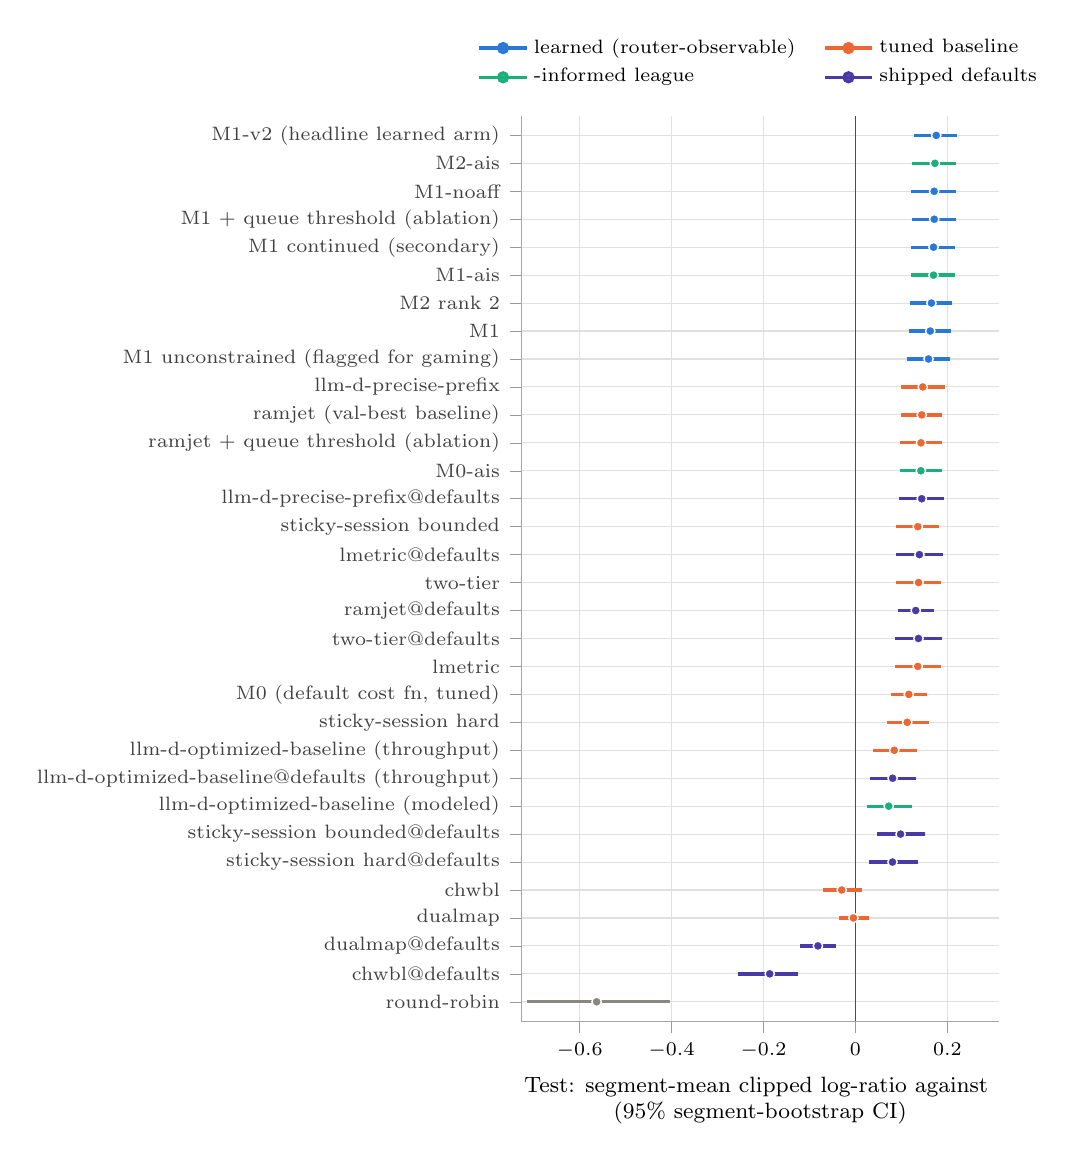
\begin{tikzpicture}
\begin{axis}[
  scale only axis, width=0.5\linewidth, height=11.5cm,
  y dir=reverse, ymin=-0.7, ymax=31.7,
  ytick={0,1,2,3,4,5,6,7,8,9,10,11,12,13,14,15,16,17,18,19,20,21,22,23,24,25,26,27,28,29,30,31}, yticklabels={{M1-v2 (headline learned arm)},{M2-ais},{M1-noaff},{M1 + queue threshold (ablation)},{M1 continued (secondary)},{M1-ais},{M2 rank 2},{M1},{M1 unconstrained (flagged for gaming)},{llm-d-precise-prefix},{ramjet (val-best baseline)},{ramjet + queue threshold (ablation)},{M0-ais},{llm-d-precise-prefix@defaults},{sticky-session bounded},{lmetric@defaults},{two-tier},{ramjet@defaults},{two-tier@defaults},{lmetric},{M0 (default cost fn, tuned)},{sticky-session hard},{llm-d-optimized-baseline (throughput)},{llm-d-optimized-baseline@defaults (throughput)},{llm-d-optimized-baseline (modeled)},{sticky-session bounded@defaults},{sticky-session hard@defaults},{chwbl},{dualmap},{dualmap@defaults},{chwbl@defaults},{round-robin}},
  yticklabel style={font=\scriptsize, text=black!75}, xticklabel style={font=\scriptsize},
  scaled x ticks=false, xticklabel style={/pgf/number format/fixed},
  tick align=outside, tick style={black!40}, axis line style={black!35},
  axis x line*=bottom, axis y line*=left,
  xmajorgrids, ymajorgrids, grid style={black!12, line width=0.4pt},
  enlarge x limits={abs=0.012},
  xmax=0.3,
  xlabel={Test: segment-mean clipped log-ratio against $\piref$\\(95\% segment-bootstrap CI)}, xlabel style={font=\footnotesize, align=center},
  legend style={font=\scriptsize, draw=none, fill=white, fill opacity=0.85, text opacity=1, at={(0.5,1.02)}, anchor=south, legend columns=2, /tikz/every even column/.append style={column sep=8pt}},
  legend cell align=left,
  clip=false,
]
\addlegendimage{color={rgb,255:red,42;green,120;blue,214}, line width=1.2pt, mark=*, mark size=1.6pt}
\addlegendentry{learned (router-observable)}
\addlegendimage{color={rgb,255:red,235;green,104;blue,52}, line width=1.2pt, mark=*, mark size=1.6pt}
\addlegendentry{tuned baseline}
\addlegendimage{color={rgb,255:red,27;green,175;blue,122}, line width=1.2pt, mark=*, mark size=1.6pt}
\addlegendentry{\ais{}-informed league}
\addlegendimage{color={rgb,255:red,74;green,58;blue,167}, line width=1.2pt, mark=*, mark size=1.6pt}
\addlegendentry{shipped defaults}
\draw[black!70, line width=0.6pt] (axis cs:0,-0.7) -- (axis cs:0,31.7);
% row 0: m1v2
\addplot[color={rgb,255:red,42;green,120;blue,214}, line width=1.2pt, forget plot] coordinates {(0.12703656654913123,0) (0.22176766566928766,0)};
\addplot[color={rgb,255:red,42;green,120;blue,214}, only marks, mark=*, mark size=1.7pt, mark options={draw=white, line width=0.5pt}, forget plot] coordinates {(0.17578143769993118,0)};
% row 1: m2ais
\addplot[color={rgb,255:red,27;green,175;blue,122}, line width=1.2pt, forget plot] coordinates {(0.12390968382254673,1) (0.2190776861031586,1)};
\addplot[color={rgb,255:red,27;green,175;blue,122}, only marks, mark=*, mark size=1.7pt, mark options={draw=white, line width=0.5pt}, forget plot] coordinates {(0.17286673166449287,1)};
% row 2: m1noaff
\addplot[color={rgb,255:red,42;green,120;blue,214}, line width=1.2pt, forget plot] coordinates {(0.12181314636266101,2) (0.2178070128886926,2)};
\addplot[color={rgb,255:red,42;green,120;blue,214}, only marks, mark=*, mark size=1.7pt, mark options={draw=white, line width=0.5pt}, forget plot] coordinates {(0.171190484541723,2)};
% row 3: ablam1
\addplot[color={rgb,255:red,42;green,120;blue,214}, line width=1.2pt, forget plot] coordinates {(0.12216696523587754,3) (0.21787594879862668,3)};
\addplot[color={rgb,255:red,42;green,120;blue,214}, only marks, mark=*, mark size=1.7pt, mark options={draw=white, line width=0.5pt}, forget plot] coordinates {(0.17141768706854468,3)};
% row 4: m1cont
\addplot[color={rgb,255:red,42;green,120;blue,214}, line width=1.2pt, forget plot] coordinates {(0.12109149167744096,4) (0.21576375139222648,4)};
\addplot[color={rgb,255:red,42;green,120;blue,214}, only marks, mark=*, mark size=1.7pt, mark options={draw=white, line width=0.5pt}, forget plot] coordinates {(0.169873390601464,4)};
% row 5: m1ais
\addplot[color={rgb,255:red,27;green,175;blue,122}, line width=1.2pt, forget plot] coordinates {(0.12079681370764042,5) (0.21632165247413257,5)};
\addplot[color={rgb,255:red,27;green,175;blue,122}, only marks, mark=*, mark size=1.7pt, mark options={draw=white, line width=0.5pt}, forget plot] coordinates {(0.16985691147737544,5)};
% row 6: m2r2
\addplot[color={rgb,255:red,42;green,120;blue,214}, line width=1.2pt, forget plot] coordinates {(0.11764196543662414,6) (0.21067909813185634,6)};
\addplot[color={rgb,255:red,42;green,120;blue,214}, only marks, mark=*, mark size=1.7pt, mark options={draw=white, line width=0.5pt}, forget plot] coordinates {(0.16533766169352687,6)};
% row 7: m1
\addplot[color={rgb,255:red,42;green,120;blue,214}, line width=1.2pt, forget plot] coordinates {(0.11564640892115144,7) (0.2072323368882717,7)};
\addplot[color={rgb,255:red,42;green,120;blue,214}, only marks, mark=*, mark size=1.7pt, mark options={draw=white, line width=0.5pt}, forget plot] coordinates {(0.16282326060787347,7)};
% row 8: m1u
\addplot[color={rgb,255:red,42;green,120;blue,214}, line width=1.2pt, forget plot] coordinates {(0.11143210946294681,8) (0.20470928733579627,8)};
\addplot[color={rgb,255:red,42;green,120;blue,214}, only marks, mark=*, mark size=1.7pt, mark options={draw=white, line width=0.5pt}, forget plot] coordinates {(0.1589590864709807,8)};
% row 9: llmdpp
\addplot[color={rgb,255:red,235;green,104;blue,52}, line width=1.2pt, forget plot] coordinates {(0.09861310334025862,9) (0.19389557066981786,9)};
\addplot[color={rgb,255:red,235;green,104;blue,52}, only marks, mark=*, mark size=1.7pt, mark options={draw=white, line width=0.5pt}, forget plot] coordinates {(0.14644600247013137,9)};
% row 10: ramjet
\addplot[color={rgb,255:red,235;green,104;blue,52}, line width=1.2pt, forget plot] coordinates {(0.09828279574825906,10) (0.18940257755445838,10)};
\addplot[color={rgb,255:red,235;green,104;blue,52}, only marks, mark=*, mark size=1.7pt, mark options={draw=white, line width=0.5pt}, forget plot] coordinates {(0.14422659924263834,10)};
% row 11: ablabase
\addplot[color={rgb,255:red,235;green,104;blue,52}, line width=1.2pt, forget plot] coordinates {(0.09701337309509567,11) (0.18752162803877784,11)};
\addplot[color={rgb,255:red,235;green,104;blue,52}, only marks, mark=*, mark size=1.7pt, mark options={draw=white, line width=0.5pt}, forget plot] coordinates {(0.14258951638820147,11)};
% row 12: m0ais
\addplot[color={rgb,255:red,27;green,175;blue,122}, line width=1.2pt, forget plot] coordinates {(0.09673094011801839,12) (0.18736256581018823,12)};
\addplot[color={rgb,255:red,27;green,175;blue,122}, only marks, mark=*, mark size=1.7pt, mark options={draw=white, line width=0.5pt}, forget plot] coordinates {(0.14234110495793503,12)};
% row 13: llm-d-precise-prefix@defaults
\addplot[color={rgb,255:red,74;green,58;blue,167}, line width=1.2pt, forget plot] coordinates {(0.09517248828100115,13) (0.19316619122098141,13)};
\addplot[color={rgb,255:red,74;green,58;blue,167}, only marks, mark=*, mark size=1.7pt, mark options={draw=white, line width=0.5pt}, forget plot] coordinates {(0.14420002518899536,13)};
% row 14: stickybounded
\addplot[color={rgb,255:red,235;green,104;blue,52}, line width=1.2pt, forget plot] coordinates {(0.0892680494472722,14) (0.18180551686371837,14)};
\addplot[color={rgb,255:red,235;green,104;blue,52}, only marks, mark=*, mark size=1.7pt, mark options={draw=white, line width=0.5pt}, forget plot] coordinates {(0.1356687801843924,14)};
% row 15: lmetric@defaults
\addplot[color={rgb,255:red,74;green,58;blue,167}, line width=1.2pt, forget plot] coordinates {(0.0888962775650902,15) (0.19013121389356863,15)};
\addplot[color={rgb,255:red,74;green,58;blue,167}, only marks, mark=*, mark size=1.7pt, mark options={draw=white, line width=0.5pt}, forget plot] coordinates {(0.13920811246409123,15)};
% row 16: twotier
\addplot[color={rgb,255:red,235;green,104;blue,52}, line width=1.2pt, forget plot] coordinates {(0.08787299176690117,16) (0.18657524522528626,16)};
\addplot[color={rgb,255:red,235;green,104;blue,52}, only marks, mark=*, mark size=1.7pt, mark options={draw=white, line width=0.5pt}, forget plot] coordinates {(0.13740693013546093,16)};
% row 17: ramjet@defaults
\addplot[color={rgb,255:red,74;green,58;blue,167}, line width=1.2pt, forget plot] coordinates {(0.09256592164675977,17) (0.1706439890179096,17)};
\addplot[color={rgb,255:red,74;green,58;blue,167}, only marks, mark=*, mark size=1.7pt, mark options={draw=white, line width=0.5pt}, forget plot] coordinates {(0.13120578511074651,17)};
% row 18: two-tier@defaults
\addplot[color={rgb,255:red,74;green,58;blue,167}, line width=1.2pt, forget plot] coordinates {(0.08667915681442735,18) (0.18747582618909142,18)};
\addplot[color={rgb,255:red,74;green,58;blue,167}, only marks, mark=*, mark size=1.7pt, mark options={draw=white, line width=0.5pt}, forget plot] coordinates {(0.1370835488619148,18)};
% row 19: lmetric
\addplot[color={rgb,255:red,235;green,104;blue,52}, line width=1.2pt, forget plot] coordinates {(0.08603413756550143,19) (0.18573594528663667,19)};
\addplot[color={rgb,255:red,235;green,104;blue,52}, only marks, mark=*, mark size=1.7pt, mark options={draw=white, line width=0.5pt}, forget plot] coordinates {(0.13559514926145588,19)};
% row 20: m0
\addplot[color={rgb,255:red,235;green,104;blue,52}, line width=1.2pt, forget plot] coordinates {(0.07773044867862913,20) (0.15621326507419445,20)};
\addplot[color={rgb,255:red,235;green,104;blue,52}, only marks, mark=*, mark size=1.7pt, mark options={draw=white, line width=0.5pt}, forget plot] coordinates {(0.11615259593474729,20)};
% row 21: stickyhard
\addplot[color={rgb,255:red,235;green,104;blue,52}, line width=1.2pt, forget plot] coordinates {(0.06816377714898289,21) (0.16085825155500855,21)};
\addplot[color={rgb,255:red,235;green,104;blue,52}, only marks, mark=*, mark size=1.7pt, mark options={draw=white, line width=0.5pt}, forget plot] coordinates {(0.11266423302798644,21)};
% row 22: llmdob
\addplot[color={rgb,255:red,235;green,104;blue,52}, line width=1.2pt, forget plot] coordinates {(0.037722088434720864,22) (0.1341168734355526,22)};
\addplot[color={rgb,255:red,235;green,104;blue,52}, only marks, mark=*, mark size=1.7pt, mark options={draw=white, line width=0.5pt}, forget plot] coordinates {(0.08444506901240169,22)};
% row 23: llm-d-optimized-baseline@throughput
\addplot[color={rgb,255:red,74;green,58;blue,167}, line width=1.2pt, forget plot] coordinates {(0.032531527863121475,23) (0.13140445967972386,23)};
\addplot[color={rgb,255:red,74;green,58;blue,167}, only marks, mark=*, mark size=1.7pt, mark options={draw=white, line width=0.5pt}, forget plot] coordinates {(0.08091673123958297,23)};
% row 24: llmdobm
\addplot[color={rgb,255:red,27;green,175;blue,122}, line width=1.2pt, forget plot] coordinates {(0.02409420705018775,24) (0.12316326800285125,24)};
\addplot[color={rgb,255:red,27;green,175;blue,122}, only marks, mark=*, mark size=1.7pt, mark options={draw=white, line width=0.5pt}, forget plot] coordinates {(0.07239319416774055,24)};
% row 25: sticky-bounded@defaults
\addplot[color={rgb,255:red,74;green,58;blue,167}, line width=1.2pt, forget plot] coordinates {(0.047519933441449176,25) (0.15141698741032308,25)};
\addplot[color={rgb,255:red,74;green,58;blue,167}, only marks, mark=*, mark size=1.7pt, mark options={draw=white, line width=0.5pt}, forget plot] coordinates {(0.09823089855750035,25)};
% row 26: sticky-hard@defaults
\addplot[color={rgb,255:red,74;green,58;blue,167}, line width=1.2pt, forget plot] coordinates {(0.030478380729487182,26) (0.13678912203631782,26)};
\addplot[color={rgb,255:red,74;green,58;blue,167}, only marks, mark=*, mark size=1.7pt, mark options={draw=white, line width=0.5pt}, forget plot] coordinates {(0.08055060851194569,26)};
% row 27: chwbl
\addplot[color={rgb,255:red,235;green,104;blue,52}, line width=1.2pt, forget plot] coordinates {(-0.07107827540927976,27) (0.013233178677833898,27)};
\addplot[color={rgb,255:red,235;green,104;blue,52}, only marks, mark=*, mark size=1.7pt, mark options={draw=white, line width=0.5pt}, forget plot] coordinates {(-0.029918674026883096,27)};
% row 28: dualmap
\addplot[color={rgb,255:red,235;green,104;blue,52}, line width=1.2pt, forget plot] coordinates {(-0.03664970706569164,28) (0.029651301114236972,28)};
\addplot[color={rgb,255:red,235;green,104;blue,52}, only marks, mark=*, mark size=1.7pt, mark options={draw=white, line width=0.5pt}, forget plot] coordinates {(-0.004392614792377874,28)};
% row 29: dualmap@defaults
\addplot[color={rgb,255:red,74;green,58;blue,167}, line width=1.2pt, forget plot] coordinates {(-0.1199719266490455,29) (-0.042838652965060606,29)};
\addplot[color={rgb,255:red,74;green,58;blue,167}, only marks, mark=*, mark size=1.7pt, mark options={draw=white, line width=0.5pt}, forget plot] coordinates {(-0.08165664015863246,29)};
% row 30: chwbl@defaults
\addplot[color={rgb,255:red,74;green,58;blue,167}, line width=1.2pt, forget plot] coordinates {(-0.25565759175765096,30) (-0.12579617818786643,30)};
\addplot[color={rgb,255:red,74;green,58;blue,167}, only marks, mark=*, mark size=1.7pt, mark options={draw=white, line width=0.5pt}, forget plot] coordinates {(-0.18657074945136784,30)};
% row 31: round_robin
\addplot[color={rgb,255:red,137;green,135;blue,129}, line width=1.2pt, forget plot] coordinates {(-0.7147261959541594,31) (-0.40314218613736974,31)};
\addplot[color={rgb,255:red,137;green,135;blue,129}, only marks, mark=*, mark size=1.7pt, mark options={draw=white, line width=0.5pt}, forget plot] coordinates {(-0.5631340198746552,31)};
\end{axis}
\end{tikzpicture}

  % src: CR/report/data/report_data.json comparisons.default.<policy>.all (segment_mean, ci95), drawn by
  %      scripts/make_figures.py with the table labels (formerly fig/leaderboard.png, report figure F3)
  \caption{Every test policy against $\piref$ (60 cells, 12 segments; segment means with 95\%
    segment-bootstrap intervals). Blue: router-observable learned arms; orange: tuned baselines;
    green: the \ais{}-informed league; purple: heuristics at their shipped parameters (suffix
    @defaults); grey: round-robin. The M1 row is also M1 restricted to its default-router start
    (\cref{sec:res-ladder}).}
  % prov: the report's row label for M1 was "M1 (= A12 M1-default-init)"
  \label{fig:leaderboard}
\end{figure}

% =====================================================================================
\subsection{Strata by load mode}
\label{sec:res-strata}

\Cref{tab:strata} breaks the headline down by load mode, worker count, family and transform; the
next two subsections read its worker-count, family and transform rows. Only the first row is a
test; the rest are descriptive, and per-worker-count claims would need Holm's correction, under
which every per-count $p$ is at least 0.070.
% src: CR/report/REPORT.md section 2 ("all Holm-adjusted per-N p >= 0.070")
% prov: the heading was "Strata: load mode, worker count, family and transforms"; sec:res-n and the
%       families subsection read the other strata

\begin{table}[tbp]
  \centering
  \caption{The headline by stratum, M1-v2 minus tuned \policy{ramjet}. One-sided exact
    Wilcoxon $p$ over the stratum's segments; only the first row is a test. Rows marked $\dagger$
    use the within-segment cell bootstrap.}
  \label{tab:strata}
  % GENERATED by scripts/make_tables.py from the report fragment report/data/tables/headline_strata.md.
% Do not edit; regenerate.
{\scriptsize
\begin{adjustbox}{max width=\linewidth}
\begin{tabular}{@{}lrrlrr@{}}
\toprule
Stratum & Cells & Seg. & M1-v2 $-$ ramjet [95\% CI] & Ahead & One-sided $p$ \\
\midrule
\textbf{all (pre-registered test)} & 60 & 12 & $+$0.0316 [$+$0.0150, $+$0.0501] & 10/12 & 0.0017 \\
load mode: open loop & 31 & 8 & $+$0.0281 [$+$0.0032, $+$0.0608] & 5/8 & 0.0742 \\
load mode: closed loop & 15 & 6 & $+$0.0354 [$+$0.0106, $+$0.0633] & 4/6 & 0.0781 \\
load mode: agentic lanes & 14 & 4 & $+$0.0374 [$+$0.0331, $+$0.0411] & 4/4 & 0.0625 \\
$\Nw = 2$ (unseen) & 8 & 6 & $+$0.0382 [$+$0.0138, $+$0.0660] & 6/6 & 0.0156 \\
$\Nw = 4$ (train count) & 13 & 7 & $+$0.0548 [$+$0.0110, $+$0.1085] & 5/7 & 0.0391 \\
$\Nw = 6$ (selection-exposed) & 7 & 6 & $+$0.0296 [$-$0.0004, $+$0.0655] & 3/6 & 0.2188 \\
$\Nw = 8$ (train count) & 17 & 8 & $+$0.0427 [$+$0.0140, $+$0.0788] & 7/8 & 0.0117 \\
$\Nw = 16$ (unseen) & 7 & 6 & $+$0.0288 [$+$0.0096, $+$0.0484] & 5/6 & 0.0312 \\
$\Nw = 32$ (unseen) & 8 & 6 & $+$0.0240 [$+$0.0079, $+$0.0416] & 6/6 & 0.0156 \\
unseen $\Nw$ (2, 16, 32) & 23 & 7 & $+$0.0342 [$+$0.0159, $+$0.0515] & 7/7 & 0.0078 \\
seen $\Nw$ (4, 8) & 30 & 12 & $+$0.0346 [$+$0.0123, $+$0.0610] & 9/12 & 0.0081 \\
transforms beyond train ranges & 10 & 7 & $+$0.0250 [$+$0.0071, $+$0.0443] & 4/7 & 0.1094 \\
family: Mooncake & 25 & 2 & $+$0.0505 [$+$0.0368, $+$0.0645]$^{\dagger}$ & 2/2 & 0.2500 \\
family: FAST25 conversation & 3 & 2 & $+$0.3868 [$+$0.2857, $+$0.4879]$^{\dagger}$ & 2/2 & 0.2500 \\
family: FAST25 synthetic & 3 & 2 & $+$0.0304 [$+$0.0164, $+$0.0443]$^{\dagger}$ & 2/2 & 0.2500 \\
family: sessions & 15 & 4 & $+$0.0001 [$-$0.0001, $+$0.0004] & 2/4 & 0.4375 \\
family: AgentX & 14 & 4 & $+$0.0374 [$+$0.0331, $+$0.0411] & 4/4 & 0.0625 \\
\bottomrule
\end{tabular}
\end{adjustbox}}

\end{table}

M1-v2 leads in all three load modes, by $+0.028$ in open loop, $+0.035$ in closed loop and $+0.037$
in agentic lanes, none significant on its own ($p$ 0.06 to 0.08); \cref{tab:mode} in
\cref{app:tables} gives selected policies by load mode. AgentX ran only in agentic lanes.
% src: generated/strata.tex rows load mode; generated/mode_vs_ramjet.tex, generated/mode_vs_default.tex
%      (tab:mode); CR/cells/{train,val,test}.jsonl (family x load.mode: every AgentX cell, and only
%      AgentX, is in agentic lanes; 8, 4 and 14 cells)

\subsection{Held-out worker counts}
\label{sec:res-n}

\begin{figure}[tbp]
  \centering
  % GENERATED by scripts/make_figures.py from report/data/report_data.json. Do not edit; regenerate.
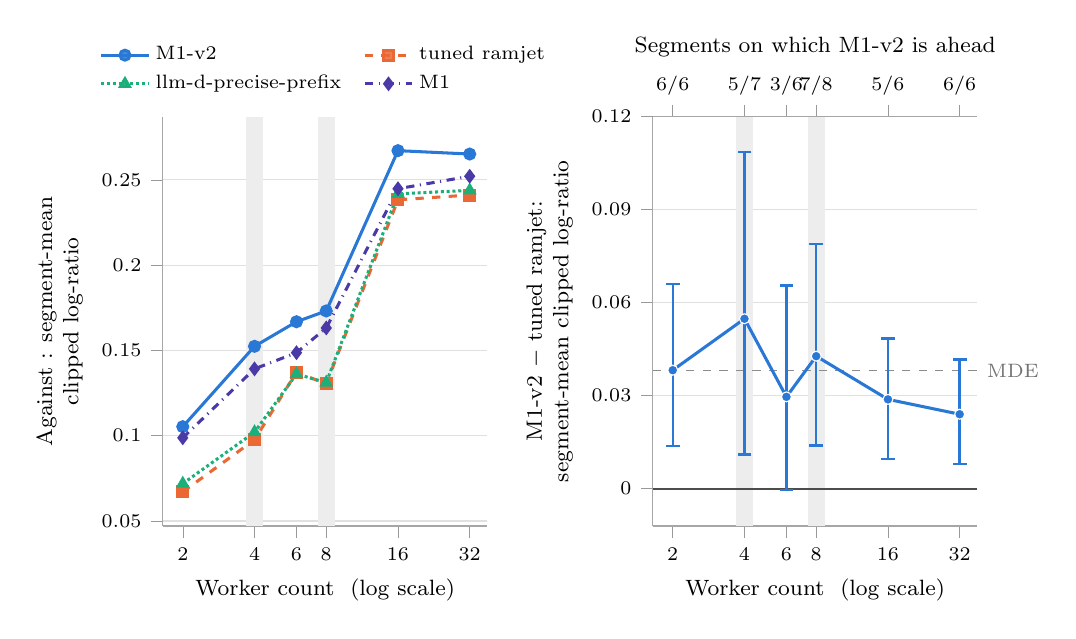
\begin{tikzpicture}
\begin{axis}[
  name=nleft, width=0.34\linewidth, height=5.2cm,
  scale only axis,
  tick label style={font=\scriptsize}, label style={font=\footnotesize, align=center},
  scaled ticks=false, tick label style={/pgf/number format/fixed},
  tick align=outside, tick style={black!40}, axis line style={black!35},
  axis x line*=bottom, axis y line*=left,
  grid style={black!12, line width=0.4pt},
  legend style={font=\scriptsize, draw=none, fill=white, fill opacity=0.85, text opacity=1},
  legend cell align=left,
  xmode=log, log basis x=2, xmin=1.65, xmax=38,
  xtick={2,4,6,8,16,32}, xticklabels={2,4,6,8,16,32}, xminorticks=false,
  xlabel={Worker count $\Nw$ (log scale)},
  ymajorgrids,
  ylabel={Against $\piref$: segment-mean\\clipped log-ratio},
  legend style={at={(0.5,1.03)}, anchor=south, legend columns=2, /tikz/every even column/.append style={column sep=6pt}},
]
\fill[black!7] ({axis cs:3.6807506024995003,0} |- {rel axis cs:0,0}) rectangle ({axis cs:4.346939450104232,0} |- {rel axis cs:0,1});
\fill[black!7] ({axis cs:7.3615012049990005,0} |- {rel axis cs:0,0}) rectangle ({axis cs:8.693878900208464,0} |- {rel axis cs:0,1});
% data: vs_default.m1v2
\addplot[color={rgb,255:red,42;green,120;blue,214}, solid, line width=1.1pt, mark=*, mark size=1.8pt, mark options={solid}] coordinates {(2.0,0.10529501096821288) (4.0,0.15242254036422193) (6.0,0.1668313049122252) (8.0,0.17316070390741592) (16.0,0.2671509076008782) (32.0,0.26516589532107004)};
\addlegendentry{M1-v2}
% data: vs_default.ramjet
\addplot[color={rgb,255:red,235;green,104;blue,52}, dashed, line width=1.1pt, mark=square*, mark size=1.8pt, mark options={solid}] coordinates {(2.0,0.06707443797134567) (4.0,0.09761725816198387) (6.0,0.13720277685467883) (8.0,0.13041631200744147) (16.0,0.2383279917374654) (32.0,0.24114203440810641)};
\addlegendentry{tuned \policy{ramjet}}
% data: vs_default.llmdpp
\addplot[color={rgb,255:red,27;green,175;blue,122}, densely dotted, line width=1.1pt, mark=triangle*, mark size=1.8pt, mark options={solid}] coordinates {(2.0,0.07189553916778706) (4.0,0.10206134188834358) (6.0,0.13618046231011913) (8.0,0.1311275495274687) (16.0,0.24183447602932287) (32.0,0.2438565952246938)};
\addlegendentry{\policy{llm-d-precise-prefix}}
% data: vs_default.m1
\addplot[color={rgb,255:red,74;green,58;blue,167}, dashdotted, line width=1.1pt, mark=diamond*, mark size=1.8pt, mark options={solid}] coordinates {(2.0,0.09875997421164102) (4.0,0.13917749407109334) (6.0,0.14867616361482291) (8.0,0.16317282053987414) (16.0,0.24481944301106787) (32.0,0.25212463174528565)};
\addlegendentry{M1}
\end{axis}
\begin{axis}[
  at={(nleft.south east)}, anchor=south west, xshift=2.1cm,
  width=0.34\linewidth, height=5.2cm, ymin=-0.012, ymax=0.12,
  scale only axis,
  tick label style={font=\scriptsize}, label style={font=\footnotesize, align=center},
  scaled ticks=false, tick label style={/pgf/number format/fixed},
  tick align=outside, tick style={black!40}, axis line style={black!35},
  axis x line*=bottom, axis y line*=left,
  grid style={black!12, line width=0.4pt},
  legend style={font=\scriptsize, draw=none, fill=white, fill opacity=0.85, text opacity=1},
  legend cell align=left,
  xmode=log, log basis x=2, xmin=1.65, xmax=38,
  xtick={2,4,6,8,16,32}, xticklabels={2,4,6,8,16,32}, xminorticks=false,
  xlabel={Worker count $\Nw$ (log scale)},
  ymajorgrids,
  ylabel={M1-v2 $-$ tuned \policy{ramjet}:\\segment-mean clipped log-ratio},
  ytick={0,0.03,0.06,0.09,0.12}, clip=false,
]
\fill[black!7] ({axis cs:3.6807506024995003,0} |- {rel axis cs:0,0}) rectangle ({axis cs:4.346939450104232,0} |- {rel axis cs:0,1});
\fill[black!7] ({axis cs:7.3615012049990005,0} |- {rel axis cs:0,0}) rectangle ({axis cs:8.693878900208464,0} |- {rel axis cs:0,1});
\draw[black!70, line width=0.6pt] ({rel axis cs:0,0} |- {axis cs:0,0.0}) -- ({rel axis cs:1,0} |- {axis cs:0,0.0});
\draw[black!45, line width=0.5pt, dashed] ({rel axis cs:0,0} |- {axis cs:0,0.03815}) -- ({rel axis cs:1,0} |- {axis cs:0,0.03815});
\node[anchor=west, font=\scriptsize, text=black!55] at ({rel axis cs:1,0} |- {axis cs:0,0.03815}) {MDE};
% data: vs_ramjet.ci.N2
\addplot[color={rgb,255:red,42;green,120;blue,214}, line width=0.9pt, mark=-, mark size=2.5pt, forget plot] coordinates {(2.0,0.01379630847680984) (2.0,0.06596507596701744)};
% data: vs_ramjet.ci.N4
\addplot[color={rgb,255:red,42;green,120;blue,214}, line width=0.9pt, mark=-, mark size=2.5pt, forget plot] coordinates {(4.0,0.01103680992682553) (4.0,0.10854519952877277)};
% data: vs_ramjet.ci.N6
\addplot[color={rgb,255:red,42;green,120;blue,214}, line width=0.9pt, mark=-, mark size=2.5pt, forget plot] coordinates {(6.0,-0.00036923336357217357) (6.0,0.06546849679810222)};
% data: vs_ramjet.ci.N8
\addplot[color={rgb,255:red,42;green,120;blue,214}, line width=0.9pt, mark=-, mark size=2.5pt, forget plot] coordinates {(8.0,0.013973978587489277) (8.0,0.07882742248882066)};
% data: vs_ramjet.ci.N16
\addplot[color={rgb,255:red,42;green,120;blue,214}, line width=0.9pt, mark=-, mark size=2.5pt, forget plot] coordinates {(16.0,0.009604036878807847) (16.0,0.048368823083775964)};
% data: vs_ramjet.ci.N32
\addplot[color={rgb,255:red,42;green,120;blue,214}, line width=0.9pt, mark=-, mark size=2.5pt, forget plot] coordinates {(32.0,0.007946861894933812) (32.0,0.041617767312250774)};
% data: vs_ramjet.mean
\addplot[color={rgb,255:red,42;green,120;blue,214}, line width=1.1pt, mark=*, mark size=1.8pt, mark options={draw=white, line width=0.4pt}] coordinates {(2.0,0.03822057299686717) (4.0,0.054805282202238036) (6.0,0.029628528057546417) (8.0,0.04274439189997442) (16.0,0.02882291586341278) (32.0,0.024023860912963633)};
\end{axis}
\begin{axis}[
  at={(nleft.south east)}, anchor=south west, xshift=2.1cm,
  width=0.34\linewidth, height=5.2cm, ymin=-0.012, ymax=0.12,
  scale only axis, xmode=log, log basis x=2, xmin=1.65, xmax=38,
  axis x line*=top, axis y line=none, tick align=outside, tick style={black!40},
  axis line style={black!35}, xminorticks=false,
  tick label style={font=\scriptsize}, label style={font=\footnotesize},
  xtick={2,4,6,8,16,32},
  xticklabels={6/6,5/7,3/6,7/8,5/6,6/6},
  xlabel={Segments on which M1-v2 is ahead},
]
\addplot[draw=none, forget plot] coordinates {(2,0)};
\end{axis}
\end{tikzpicture}

  % src: CR/report/data/report_data.json comparisons.default.<m1v2|ramjet|llmdpp|m1>.N:<n>.segment_mean
  %      and comparisons.ramjet.m1v2.N:<n> (segment_mean, ci95, segments_ahead, segments), drawn by
  %      scripts/make_figures.py (formerly fig/worker_count_extrapolation.png, report figure F2)
  \caption{Worker-count extrapolation on test. Left: segment means
    against $\piref$ by $\Nw$ (intervals in \cref{tab:N-default} in \cref{app:tables}).
    Right: M1-v2 minus tuned \policy{ramjet} by $\Nw$, with 95\% segment-bootstrap intervals and,
    on the top axis, the segments on which M1-v2 is ahead; dashed: the MDE.
    Shaded: the train counts 4 and 8. Each $\Nw$ holds different cells, and loads are matched to
    $\piref$'s knee at each $\Nw$, not to a fixed per-worker rate.}
  \label{fig:n-extrapolation}
\end{figure}

Every learned arm was trained on $\Nw \in \{4, 8\}$ only and runs unchanged at any $\Nw$, because its
utility is per worker and its features are set-size invariant (\cref{sec:set-size}).
\Cref{fig:n-extrapolation} plots the test results by $\Nw$.
\begin{itemize}
  \item \textbf{The margin persists at unseen worker counts.} Over \policy{ramjet} it is positive at
    every $\Nw$: $+0.038$ at $\Nw = 2$, $+0.029$ at 16 and $+0.024$ at 32 (\cref{tab:N-ramjet} in
    \cref{app:tables}). Over
    the 7 segments with cells at unseen counts it is ahead on all 7 ($+0.034$, uncorrected $p$
    0.008); this stratum was not pre-registered as a test.
  \item \textbf{No regression.} The pre-registered no-regression check holds at $\Nw = 2$, 16 and 32
    against both \policy{ramjet} and $\piref$: the lower end of the interval exceeds
    $-\ln 1.005$.
  \item \textbf{Gains over the default grow with $\Nw$} for every cache-aware policy, M1-v2's from
    $+0.105$ at $\Nw = 2$ to $+0.27$ at 16 and 32, but the learned margin over \policy{ramjet} does
    not grow at the unseen large counts.
  \item \textbf{$\Nw = 6$ is selection-exposed} and the weakest stratum: 3 of 6 segments ahead,
    $p$ 0.219.
  \item \textbf{The curve is not a pure $\Nw$ effect.} Each $\Nw$ holds different cells and
    segments, and with loads matched to $\piref$'s knee per $\Nw$ the per-worker load varies 1.2 to
    1.9 times across $\Nw$. A per-worker-matched extrapolation was not run.
\end{itemize}
% src: generated/N_vs_ramjet.tex, generated/strata.tex (unseen_N 7/7, p 0.0078; N:6 3/6, p 0.2188);
%      CR/facts/test_results.json parity_and_no_regression; CR/report/REPORT.md section 4;
%      CR/audits/calibration/independent-rerun-r1.md F3 (1.2-1.9x)
M1-v2's gain rises with cache pressure on the 22 open-loop Mooncake and FAST25 test cells (Spearman
$\rho$ 0.79 against $\piref$, 0.71 against \policy{ramjet}), a descriptive trend confounded with load
level (\cref{app:results}).
% src: CR/report/REPORT.md section 4 ("On the 22 open-loop Mooncake and FAST25 test cells ... Spearman
%      rho 0.79 against default and 0.71 against ramjet ... Pressure is confounded with load level")

\subsection{Families and transforms}

By family (\cref{tab:family-ramjet} in \cref{app:tables}; descriptive, with 2 to 4 segments each),
the margin is largest on the FAST25 conversation cells ($+0.387$), a family no policy was trained on; those three cells carry about 35\% of M1-v2's
cell-mean gain, and their request-count gains ($+0.48$, $+0.49$, $+0.08$) contrast with token-weighted
deltas of $+0.02$, $-0.15$ and $+0.02$ (\cref{sec:gaming}). On Mooncake the lead is $+0.050$, on
AgentX $+0.037$ with all four segments ahead, and on FAST25 synthetic $+0.030$. Sessions sit at
ceiling at the calibrated SLO: every strong policy serves nearly every in-window session request
well, so the four session segments tie. The ten cells with transforms beyond the train ranges show
$+0.025$ with 4 of 7 segments ahead ($p$ 0.109), so generalization to held-out transform values is
not established. \Cref{tab:holdout} in \cref{app:tables} gives selected policies at unseen and seen
worker counts and on the transform cells.
% src: generated/family_vs_ramjet.tex; CR/report/REPORT.md section 3.3 (35%, +0.48/+0.49/+0.08 vs
%      +0.02/-0.15/+0.02); generated/strata.tex (transform_extrapolation +0.0250, 4/7, 0.1094);
%      generated/holdout_vs_{ramjet,default}.tex (tab:holdout columns)

% =====================================================================================
\subsection{The model ladder and the ablations}
\label{sec:res-ladder}

\begin{table}[tbp]
  \centering
  \caption{The model ladder. Val $k_{0..2}$ and Val $k_{3..10}$: mean clipped log-ratio against
    $\piref$ on the selection replicates and on the fresh validation replicates. Test against $\piref$
    is a mean over cells; test against tuned \policy{ramjet} is a segment mean with its 95\% interval
    and one-sided $p$. \Cref{tab:leaderboard-full} in \cref{app:tables} gives the restart and generation at
    which each configuration was selected.}
  % prov: the selected restart and generation moved out of the main text; tab:leaderboard-full has them
  \label{tab:ladder-results}
  % GENERATED by scripts/make_tables.py from the report fragment report/data/tables/ladder.md.
% Do not edit; regenerate.
{\scriptsize
\begin{adjustbox}{max width=\linewidth}
\begin{tabular}{@{}P{0.25\linewidth}rrrlr@{}}
\toprule
Rung & Val $k_{0..2}$ & Val $k_{3..10}$ & Test vs $\piref$ & Test vs ramjet [95\% CI] & $p$ \\
\midrule
M0 & 0.1334 & 0.1326 & $+$0.1102 & $-$0.0281 [$-$0.0439, $-$0.0137] & 0.9993 \\
M1 & 0.1660 & 0.1656 & $+$0.1741 & $+$0.0186 [$+$0.0013, $+$0.0378] & 0.0549 \\
M1 continued ($+$400 evals) & 0.1704 & 0.1672 & $+$0.1811 & $+$0.0256 [$+$0.0090, $+$0.0437] & 0.0212 \\
M2 rank 2 & 0.1688 & 0.1677 & $+$0.1774 & $+$0.0211 [$+$0.0043, $+$0.0406] & 0.0549 \\
M1-noaff & 0.1682 & 0.1692 & $+$0.1821 & $+$0.0270 [$+$0.0109, $+$0.0443] & 0.0134 \\
M1 + queue threshold (ablation) & 0.1690 & 0.1684 & $+$0.1819 & $+$0.0272 [$+$0.0115, $+$0.0444] & 0.0171 \\
M1-v2 & 0.1767 & 0.1783 & $+$0.1877 & $+$0.0316 [$+$0.0150, $+$0.0501] & 0.0017 \\
M1 unconstrained (flagged for gaming) & 0.1636 & n/a & $+$0.1687 & $+$0.0147 [$+$0.0032, $+$0.0284] & 0.0386 \\
M0-ais & 0.1410 & 0.1397 & $+$0.1313 & $-$0.0019 [$-$0.0086, $+$0.0048] & 0.6890 \\
M1-ais & 0.1731 & 0.1718 & $+$0.1810 & $+$0.0256 [$+$0.0113, $+$0.0423] & 0.0012 \\
M2-ais & 0.1751 & 0.1735 & $+$0.1837 & $+$0.0286 [$+$0.0138, $+$0.0458] & 0.0005 \\
\bottomrule
\end{tabular}
\end{adjustbox}}

\end{table}

\Cref{tab:ladder-results} and the rung-to-rung comparisons of \cref{tab:ladder-pairs}
(\cref{app:results}, which also plots the ladder in \cref{fig:ladder}) read as follows.
\begin{itemize}
  \item \textbf{M0 $\to$ M1 is the one clear step.} Learning over the default cost's features beats
    tuning the default cost's knobs: $+0.047$ per segment, 11 of 12 segments ahead.
  \item \textbf{M1 is the sign-constrained re-run.} The first, unconstrained M1 gamed the objective
    (\cref{sec:gaming}); it is reported only as a flagged secondary row, and it is weaker on test.
    % prov: "tier-A M1"
  \item \textbf{M1 $\to$ M2 rank 2: no gain.} The context term adds $+0.0025$ on test (6 of 12
    segments) and does not beat M1 continued for the same added 400 evaluations ($-0.0045$). The
    pre-registered gate for ranks 3 and 4 failed: M2 rank 2 minus the better of M1 and M1 continued
    was $-0.0016$ on validation, against an MDE of 0.038, so ranks 3 and 4 were not run. M3 (nested
    logit) was never built, since this deployment has no nests.
  \item \textbf{M1 $\to$ M1-v2 is the step that passes.} The extended feature set, with log,
    set-relative, interaction and prefill-attention terms, beats M1 by $+0.013$ on 11 of 12 segments
    ($p$ 0.0034). The originally planned M1 and M2 alone do \emph{not} pass against \policy{ramjet}
    on test ($p$ 0.055 each); the passing arm is a redesign made after the pilot, on validation
    evidence (\cref{sec:res-fairness}).
  \item \textbf{The queue-threshold ablation: nothing measurable.} It tunes the router's queue
    threshold jointly with a policy (\cref{sec:ablations}). Against their counterparts without it,
    the learned arm with the threshold is $+0.0015$ ($p$ 0.055, against M1
    continued) and \policy{ramjet} with it is $-0.0016$, and removing the tuned threshold after the
    fact changes their validation scores by $+0.0001$ and $-0.0006$.
  \item \textbf{Session affinity.} M1-noaff, retrained without $\theta_6$, is not worse than M1
    on test ($+0.0084$, $p$ 0.21), and zeroing $\theta_6$ in the selected M1 changes its validation
    score by $-0.0010$. Under router-state lag, M1 minus M1-noaff stays between $-0.008$ and
    $-0.005$, so the hypothesis that affinity gains value as the router's state goes stale is not
    supported. For M1-v2, zeroing $\theta_6$ changes the validation score by $+0.0005$.
    % prov: A15 (M1-noaff)
  \item \textbf{Initialization.} The selected M1 came from the s1 restart, the default router,
    so the registered secondary finalist, M1 restricted to its default start, is the same policy as
    M1.
    % prov: A12, the "M1-default-init" row
    M1-v2 also came from s1; its informed restarts s2 (the behavior clone) and s3 (the faithful LMetric point) reached 0.1609 and
    0.1724 on the selection replicates, against s1's 0.1767.
\end{itemize}
% src: generated/ladder_pairs.tex and generated/ladder.tex; CR/facts/tierBC.json m2_rank3_4_gate
%      (via REPORT section 5: -0.0016 vs MDE 0.038), tier_c_final_i9 (q removed +0.00010 / -0.00064);
%      CR/facts/test_results.json secondary.m1noaff_vs_m1 (+0.008367, p 0.2119), m1_vs_ramjet and
%      m2r2_vs_ramjet (p 0.0549), m1v2_vs_m1 (+0.012958, 11/12, p 0.003418), m1_A12_note;
%      CR/facts/robustness.json a15_affinity_under_lag; CR/audits/final/refute-headline-2.md
%      (M1-v2 theta6 = 0: +0.0005); CR/report/REPORT.md section 5 (restart bests)

% =====================================================================================
\subsection{What M1-v2 learned}
\label{sec:res-coefficients}

The shipped artifact is one policy YAML: \lc{} with \code{feature\_set: v2}, $\temp = 0$,
\code{tie\_break: one\_draw} and the 23 coefficients of \cref{tab:coef-m1v2}. It reads no \ais{}
signal; a decision costs $O(\Nw\dfeat)$ with $\dfeat = 23$. We read the
coefficients through standardized magnitudes and ablations, not raw values: \cref{tab:coef-m1v2}
scales each $\theta_f$ by the feature's within-candidate-set standard deviation on train, so
$\theta_f\,\mathrm{sd}_f$ is the utility change for a typical difference between two candidates. The
anchor, the default cost per request block, has $\theta_0\,\mathrm{sd}_0 = -6.51$
(\cref{fig:coef} in \cref{app:results} plots the nonzero terms).
% src: CR/facts/finalists.json headline.learned.spec; CR/report/REPORT.md section 6 (sd on train from
%      CR/runs/phase2/m1v2/prep.json)
% prov: "Following LR-15" (reading coefficients through standardized magnitudes and ablations)

\begin{table}[tbp]
  \centering
  \caption{M1-v2's coefficients. sd$_f$: pooled within-candidate-set standard deviation
    of feature $f$ on train; constraint: the sign rule of \cref{sec:sign-constraint}.}
  \label{tab:coef-m1v2}
  % GENERATED by scripts/make_tables.py from the report fragment report/data/tables/coef_m1v2.md.
% Do not edit; regenerate.
{\scriptsize
\begin{adjustbox}{max width=\linewidth}
\begin{tabular}{@{}rlrrrl@{}}
\toprule
$f$ & Feature & $\theta_f$ & sd$_f$ & $\theta_f\,\mathrm{sd}_f$ & Constraint \\
\midrule
0 & \code{default\_logit\_scaled} & $-$1 & 6.51 & $-$6.510 & pinned $-$1 \\
1 & \code{overlap\_frac} & $+$5.034 & 0.2561 & $+$1.289 & free \\
2 & \code{new\_prefill\_tokens\_k} & $+$1.275 & 0.3519 & $+$0.449 & free \\
3 & \code{active\_prefill\_tokens\_k} & $-$0.2811 & 1.285 & $-$0.361 & $\leq$ 0 \\
4 & \code{kv\_load\_frac} & $+$0 & 0.08438 & $+$0.000 & $\leq$ 0 \\
5 & \code{active\_requests\_s} & $-$2.146 & 0.06 & $-$0.129 & $\leq$ 0 \\
6 & \code{session\_affinity} & $+$1.391 & 0.3244 & $+$0.451 & free \\
7 & \code{isl\_x\_prefill\_load} & $+$0 & 2.13 & $+$0.000 & $\leq$ 0 \\
8 & \code{log\_ptok} & $+$0 & 1.156 & $+$0.000 & $\leq$ 0 \\
9 & \code{log\_new\_prefill} & $-$0.9276 & 0.8219 & $-$0.762 & free \\
10 & \code{log\_bs} & $+$0 & 0.2708 & $+$0.000 & $\leq$ 0 \\
11 & \code{hash\_home} & $-$1.582 & 0.4668 & $-$0.738 & free \\
12 & \code{kv\_load\_ratio} & $+$0 & 0.2377 & $+$0.000 & $\leq$ 0 \\
13 & \code{active\_prefill\_ratio} & $+$0 & 0.9491 & $+$0.000 & $\leq$ 0 \\
14 & \code{active\_requests\_ratio} & $-$0.348 & 0.2576 & $-$0.090 & $\leq$ 0 \\
15 & \code{kv\_load\_below\_frac} & $+$0 & 0.2817 & $+$0.000 & $\leq$ 0 \\
16 & \code{active\_prefill\_below\_frac} & $-$1.326 & 0.2398 & $-$0.318 & $\leq$ 0 \\
17 & \code{active\_requests\_below\_frac} & $-$2.617 & 0.267 & $-$0.699 & $\leq$ 0 \\
18 & \code{kv\_load\_excess} & $+$0 & 0.05047 & $+$0.000 & $\leq$ 0 \\
19 & \code{active\_prefill\_excess} & $+$0 & 0.9154 & $+$0.000 & $\leq$ 0 \\
20 & \code{active\_requests\_excess} & $-$5.845 & 0.03463 & $-$0.202 & $\leq$ 0 \\
21 & \code{new\_prefill\_x\_requests} & $-$16.79 & 0.1268 & $-$2.128 & $\leq$ 0 \\
22 & \code{prefill\_attn} & $-$0.2967 & 0.2846 & $-$0.084 & free \\
\bottomrule
\end{tabular}
\end{adjustbox}}

\end{table}

\begin{enumerate}
  \item \textbf{The default router plus corrections.} $\theta_0 = -1$ dominates; every learned term
    is a fraction of the anchor's spread.
  \item \textbf{Uncached prefill costs more the busier the worker.} The largest learned term is
    \code{new\_prefill\_x\_requests} ($\theta_{21}\,\mathrm{sd}_{21} = -2.13$). With $\theta_2$, the
    linear weight on uncached prefill is $+1.275 - 0.525 \times$(active requests) per 8K tokens,
    negative on any worker with three or more active requests: uncached work is steered to near-idle
    workers, while cache affinity is kept on lightly loaded ones. Zeroing $\theta_{21}$ costs 0.018 on
    validation (13 of 14 cells worse), and the fairness audit attributes M1-v2's increment over the
    in-class LMetric heuristic to this term.
  \item \textbf{Cache terms reward hits beyond the default's credit.} \code{overlap\_frac}
    ($+1.29$ per sd) and the log of uncached prefill ($-0.76$ per sd) both favor the worker holding
    more of the prompt; the log term rewards near-complete hits most. Zeroing $\theta_1$ alone costs
    only 0.002 on validation: overlap is largely redundant with the anchor and the prefill terms.
  \item \textbf{Rank-like load terms do the balancing.} The set-relative terms
    \code{active\_requests\_below\_frac} ($-0.70$) and \code{active\_prefill\_below\_frac} ($-0.32$),
    with request excess and ratio, outweigh the absolute load terms ($-0.36$ and $-0.13$). LMetric's
    own product terms (\code{log\_ptok}, \code{log\_bs}) are 0 in the selected policy.
  \item \textbf{Session and prefix-home terms are unneeded.} \code{session\_affinity} ($+0.45$) and
    \code{hash\_home} ($-0.74$, a mild avoidance of the prefix's rendezvous pair) can each be zeroed
    with no validation loss ($+0.0005$ and $+0.0010$), so the policy depends on neither session IDs
    nor rendezvous homes.
\end{enumerate}
% src: CR/report/REPORT.md section 6 interpretation (items 1-5); CR/audits/final/refute-headline-2.md
%      (theta21 = 0: -0.0178; theta6 = 0 +0.0005; theta11 = 0 +0.0010)

The \code{v1} arms agree on a simpler structure (\cref{tab:coef-v1} in \cref{app:tables}): a strong extra
overlap credit ($\theta_1\,\mathrm{sd}_1$ of $+4.2$ to $+4.9$) and a strong penalty on active requests
($-2.1$ to $-2.9$) on top of the default. The unconstrained M1 used overlap and request weights about
3.5 to 3.7 times larger and a positive $\theta_7$, the gaming pattern of \cref{sec:gaming}.
% src: CR/report/REPORT.md section 6 ("The v1 arms ...")

% =====================================================================================
\subsection{Robustness}
\label{sec:res-robustness}

\begin{table}[tbp]
  \centering
  \caption{The headline under perturbations and alternative SLOs. ``Nominal $\Ezero$''
    scores timing-perturbed replays against the unperturbed $\Ezero$; ``$\Ezero'$'' uses the
    perturbation-consistent reference (\cref{sec:robustness}). $s$: speedup; $d$: decode speedup.
    $\kendall$-b compares the condition's ranking with the nominal ranking, over the 17 robustness
    finalists for lag and timing and over all 32 non-default policies for SLO variants. The last row
    is the token-weighted secondary metric.}
  \label{tab:robustness}
  % prov: the last row is A19
  % GENERATED by scripts/make_tables.py from the report fragment report/data/tables/robustness.md.
% Do not edit; regenerate.
{\scriptsize
\begin{adjustbox}{max width=\linewidth}
\begin{tabular}{@{}llrrrl@{}}
\toprule
Condition & M1-v2 $-$ ramjet [95\% CI] & Ahead & $p$ & $\kendall$-b & Rank M1-v2 / ramjet \\
\midrule
nominal & $+$0.0316 [$+$0.0150, $+$0.0501] & 10/12 & 0.0017 & 1.000 & 1 / 7 of 17 \\
lag 10 ms & $+$0.0312 [$+$0.0139, $+$0.0508] & 9/12 & 0.0081 & 0.950 & 1 / 7 of 17 \\
lag 50 ms & $+$0.0288 [$+$0.0125, $+$0.0477] & 10/12 & 0.0024 & 0.950 & 1 / 6 of 17 \\
lag 200 ms & $+$0.0304 [$+$0.0135, $+$0.0497] & 9/12 & 0.0061 & 0.917 & 1 / 7 of 17 \\
s0.8 nominal E0 & $+$0.0790 [$+$0.0042, $+$0.1666] & 8/12 & 0.1167 & 0.783 & 1 / 10 of 17 \\
s0.8 E0' & $+$0.0814 [$+$0.0229, $+$0.1511] & 9/12 & 0.0105 & 0.800 & 1 / 10 of 17 \\
s1.2 nominal E0 & $+$0.0151 [$+$0.0064, $+$0.0247] & 10/12 & 0.0081 & 0.950 & 1 / 6 of 17 \\
s1.2 E0' & $+$0.0219 [$+$0.0105, $+$0.0333] & 10/12 & 0.0046 & 0.950 & 1 / 6 of 17 \\
d0.8 nominal E0 & $+$0.0473 [$+$0.0131, $+$0.0872] & 9/12 & 0.0261 & 0.817 & 1 / 7 of 17 \\
d0.8 E0' & $+$0.0391 [$+$0.0145, $+$0.0691] & 10/12 & 0.0024 & 0.917 & 1 / 8 of 17 \\
d1.2 nominal E0 & $+$0.0224 [$+$0.0099, $+$0.0360] & 8/12 & 0.0134 & 0.950 & 1 / 6 of 17 \\
d1.2 E0' & $+$0.0304 [$+$0.0140, $+$0.0477] & 9/12 & 0.0105 & 0.950 & 1 / 6 of 17 \\
SLO scale 0.5 & $+$0.0716 [$-$0.0289, $+$0.1734] & 10/12 & 0.0647 & 0.544 & 1 / 13 of 32 \\
SLO scale 0.75 & $+$0.0353 [$-$0.0015, $+$0.0776] & 8/12 & 0.1167 & 0.907 & 1 / 10 of 32 \\
SLO scale 1.5 & $+$0.0156 [$+$0.0064, $+$0.0256] & 12/12 & 0.0002 & 0.956 & 1 / 10 of 32 \\
SLO scale 2.0 & $+$0.0113 [$+$0.0052, $+$0.0178] & 12/12 & 0.0002 & 0.931 & 2 / 10 of 32 \\
SLO scale 3.0 & $+$0.0120 [$+$0.0048, $+$0.0207] & 12/12 & 0.0002 & 0.919 & 2 / 10 of 32 \\
A14 itl\_only & $+$0.0089 [$+$0.0022, $+$0.0161] & 10/12 & 0.0134 & 0.879 & 1 / 16 of 32 \\
A14 e2e\_only & $+$0.0351 [$+$0.0152, $+$0.0574] & 11/12 & 0.0012 & 0.988 & 1 / 11 of 32 \\
A14 ttft\_len\_itl & $+$0.0134 [$+$0.0046, $+$0.0227] & 10/12 & 0.0105 & 0.847 & 1 / 10 of 32 \\
A14 abs\_e2e\_itl & $+$0.0189 [$+$0.0082, $+$0.0303] & 10/12 & 0.0061 & 0.891 & 1 / 15 of 32 \\
A19 good tokens (secondary) & $-$0.0092 [$-$0.0645, $+$0.0244] & 10/12 & 0.0320 & n/a & n/a \\
\bottomrule
\end{tabular}
\end{adjustbox}}

\end{table}

\Cref{tab:robustness} answers whether the ranking survives changes training never saw
(\cref{fig:robustness} in \cref{app:results} plots it).\footnote{The measurement window matters
  little: starting the window 25\% or 50\% later gives $+0.0345$ and $+0.0297$; halving or doubling
  the warm-up, or a common completion window, leaves the result unchanged on the same cells.}
% src (footnote): CR/audits/final/refute-headline-3.md (window +25%/+50%)
\begin{itemize}
  \item \textbf{Router-state lag.} At 10, 50 and \SI{200}{ms} the lead is $+0.031$, $+0.029$ and
    $+0.030$ ($p \le 0.0081$), M1-v2 stays first among the 17 robustness finalists, and the ranking's
    $\kendall$-b is 0.92 to 0.95. At lag 0 the patched replay reproduces the unpatched one per request
    (\cref{app:results}). Beyond the registered range, on validation only, \SI{1000}{ms} gives
    $+0.033$ against $+0.029$ at 0: the baselines lose more to staleness than M1-v2 does.
  \item \textbf{Engine timing.} The sign holds under speedup and decode speedup of 0.8 and 1.2, on
    both references, and with the ITL bound also rescaled the lead is $+0.022$ to $+0.080$
    ($p \le 0.0081$). Speedup 0.8 on the nominal $\Ezero$ is not significant ($p$ 0.117), a degenerate
    scoring in which no zero-reuse AgentX request can be good. The spread across conditions (0.060,
    set by speedup 0.8) exceeds the nominal effect, so by the reading rule of \cref{sec:robustness}
    the direction is robust and the magnitude is perturbation-dependent.
    % prov: LR-14 (the reading rule)
  \item \textbf{SLO scale.} The sign is positive at every scale; significance holds at 1 to 3 and is
    lost at 0.75 and 0.5. At 0.75 the four session segments reverse ($-0.014$ to $-0.042$), as they do
    at speedup 0.8 on the nominal reference, so ``sessions at ceiling'' holds only where the SLO does
    not bind. At 0.5 the scaled slowdown bound falls below 1 for AgentX, so only cache hits can be
    good there.
  \item \textbf{SLO definition (registered before the test pass).} M1-v2 ranks first under all
    four alternative definitions of a good request, and the ranking's $\kendall$-b against the
    trained SLO is 0.85 to 0.99: ITL only $+0.0089$ ($p$ 0.013), slowdown only $+0.035$ ($p$ 0.0012),
    length-scaled TTFT plus ITL $+0.013$ ($p$ 0.0105), absolute end-to-end plus ITL $+0.019$
    ($p$ 0.0061).
    % prov: A14
  \item \textbf{Simulator model.} On validation, four audit-only changes to \aisim{}'s pricing of
    mixed prefill and decode passes, which act on M1-v2's concentration mechanism, keep the lead
    between $+0.0268$ and $+0.0291$ against $+0.0290$; they bracket fidelity errors, are not
    measurements of reality and do not cover FAST25, a test-only family (\cref{app:results}).
    % src (pricing owner): CR/facts/UPSTREAM_FOLLOWUPS.md #17; appendix-caveats.tex row 13
  \item \textbf{Herding guards.} Run as variants of M1 (they were registered before M1-v2 won),
    neither a positive temperature nor restricting candidates to the prefix's hash-home pair helps,
    and no herding failure of the argmax appeared under the tested lags in replay
    (\cref{app:results}).
    % src: generated/tau_hashhome.tex; CR/facts/robustness.json m1_lr14_variants; CR/report/REPORT.md
    %      section 7.2
\end{itemize}
% src: generated/robustness.tex; CR/facts/robustness.json (conditions, lag0_identity_lag_build_vs_tuning_build,
%      lr14_summary); CR/audits/final/refute-headline-3.md (lag0 448/448; lag 1000 ms val +0.0333 vs
%      +0.0290; consistent timing SLO +0.022..+0.080, p <= 0.0081; window +25%/+50%; simulator model
%      variants); CR/report/REPORT.md section 7.1

% =====================================================================================
\subsection{The \ais{}-informed league}
\label{sec:res-ais-summary}

% src: generated/ladder_pairs.tex (M2-ais - M1-v2 -0.0029, 3/12; M0-ais - M0 +0.0262);
%      CR/facts/robustness.json execution.ais_league; CR/audits/final/completeness.md F2;
%      CR/facts/UPSTREAM_FOLLOWUPS.md #15
% prov: A16 (the AIS league); the full section moved to app:ais-league, which keeps sec:res-ais
The \ais{}-informed league, whose policies may read \ais{} estimates at runtime and so can never
become the headline, adds nothing at the learned level: M2-ais trails M1-v2 by 0.0029 (3 of 12 segments ahead),
although the \ais{} load model helps the default cost ($+0.026$). The league has no lag or timing
robustness evidence and is not portable as is (\cref{sec:res-ais}).

% =====================================================================================
\subsection{Scope: the in-class heuristic and asymmetric iteration}
\label{sec:res-fairness}

Equal footing was verified from the raw tuning histories by two auditors: every tuned policy, learned
or baseline, ran three restarts of 400 evaluations with the same cells, replicates, validation
schedule, objective and reference, and the splits share no trace files. The fairness audit then found
a gap that equal budgets do not close. By design the baseline pool holds the branch's
ports as implemented, and the \policy{lmetric} port as evaluated lacks LMetric's queued-prefill term
(\cref{sec:ports}). Faithful LMetric is inside M1-v2's hypothesis class, and M1-v2's restart s3
started from default plus 20.7 times the faithful LMetric point. \Cref{tab:fairness} shows what that
heuristic does on its own.
% src: CR/audits/final/refute-headline-2.md (equal footing PASS: 48 runs, one budget signature;
%      no leakage), F1; CR/facts/fairness_in_class_heuristic.json; CR/facts/test_results.json
%      report_must_state MS-RH2-F1-table, MS-RH2-F1-increment
% prov: "By design" was "By operator decision"

\begin{table}[tbp]
  \centering\small
  \caption{The in-class heuristic. \emph{Auditor diagnostic, not pre-registered, never used for
    selection; train and validation only, the test split was not evaluated.} Mean clipped
    log-ratio against $\piref$; the last column is the margin over \policy{ramjet} on the fresh
    validation replicates, per cell and per segment.}
  \label{tab:fairness}
  % src: CR/facts/fairness_in_class_heuristic.json (via CR/report/REPORT.md section 9 table, which
  %      re-derives every value from the cache: runs/final-fix/scripts/verify_fairness.py)
  \begin{adjustbox}{max width=\linewidth}
  \begin{tabular}{@{}P{0.38\linewidth}rrrl@{}}
    \toprule
    Policy (tuning) & Train $k_{0..1}$ & Val $k_{0..2}$ & Val $k_{3..10}$ & vs ramjet on $k_{3..10}$: cell / segment \\
    \midrule
    M1-v2 ($3 \times 400$ evaluations) & 0.1851 & 0.1767 & \textbf{0.1783} & $+0.0372$ / $+0.0290$ (5 of 6) \\
    default $+$ $10\times$ faithful LMetric (8 train evaluations) & 0.1566 & 0.1609 & \textbf{0.1609} & $+0.0197$ / $+0.0179$ (4 of 6) \\
    M1-v2's s3 start, $c = 20.7$ (untuned) & 0.1566 & 0.1596 & \textbf{0.1612} & $+0.0200$ / $+0.0190$ (6 of 6) \\
    faithful LMetric alone (untuned) & 0.1466 & 0.1493 & \textbf{0.1490} & $+0.0079$ / $+0.0110$ (6 of 6) \\
    \policy{ramjet} (best of 11 tuned baselines, $3 \times 400$) & 0.1435 & 0.1420 & \textbf{0.1411} & --- \\
    \bottomrule
  \end{tabular}
  \end{adjustbox}
\end{table}

\begin{itemize}
  \item \textbf{Faithful LMetric beats every tuned baseline untuned,} on the selection replicates
    (0.1493 against at most 0.1423) and on the fresh ones (0.1490 against 0.1411).
  \item \textbf{Most of the margin is the heuristic.} Default plus faithful LMetric reproduces 53 to
    66\% of M1-v2's fresh-validation margin over \policy{ramjet}.
  \item \textbf{The learned increment} over it is about $+0.011$ per segment (standard error 0.0065,
    5 of 6 segments; $+0.017$ per cell), about 0.29 of the MDE, and it \emph{was not measured on
    test}; it sits mostly on one Mooncake validation segment.
  \item \textbf{Follow-up.} A pre-registered comparison with faithful LMetric and an SMetric-style
    baseline, each tuned with the equal budget and evaluated on fresh segments or on live runs over
    cells outside the frozen test set, has not been run and is not part of this paper.
    (The live runs of \cref{sec:live} used frozen test cells and so cannot serve it.)
  \item \textbf{The port has changed since.} After this study froze its results, the
    \policy{lmetric} port in ai-dynamo/dynamo\#15450 was fixed to count the worker's queued prefill,
    so it now scores the same product as the faithful LMetric rows above, plus its hot-spot filter.
    The fixed port was not evaluated, and the diagnostic is unchanged: its faithful rows are points
    of M1-v2's class, not the port, the tuned baselines and every \policy{lmetric} number in this
    paper are from the port before the fix, and the follow-up above has still not been run.
    % src: CR/CONTRACT.md A21; CR/facts/fairness_in_class_heuristic.json policies.lmetric_faithful
    %      (learned-choice v2, theta = -(e_log_ptok + e_log_bs): argmin (active_prefill + new_prefill) x
    %      (active_requests + 1))
\end{itemize}
% src: CR/facts/fairness_in_class_heuristic.json; CR/report/REPORT.md section 9 (increment +0.0110 per
%      segment, SE 0.0065, 5/6; cell +0.0174; mostly Mooncake w1 +0.044); CR/audits/final/fix.md (escalation)

\paragraph{Asymmetric iteration.}
The learned side was redesigned on validation evidence: multi-start initialization, the sign
constraints, and M1-v2 itself, which was written to target the pilot's weakest family, plus M2,
M1-noaff and the queue-threshold arm. The baseline side gained one arm and no new heuristic types.
Selection among the five learned arms used the same fresh-validation rule as the baselines, and the
test pass was single, so the headline $p$-value is valid for the selected arm; but the originally
planned M1 and M2 do not pass on test. Two registration choices (excluding M1 continued from the
headline candidates and including the queue-threshold \policy{ramjet} in the baseline pool) cannot be
shown to predate the fresh-validation results; both were outcome-neutral on those values, and we do
not claim strict pre-registration for them.
% src: CR/audits/final/refute-headline-2.md F2; CR/audits/final/completeness.md F5;
%      CR/audits/final/refute-headline-1.md F6; CR/report/REPORT.md section 9 ("Registration timing")
